\documentclass{article} % For LaTeX2e
\usepackage{nips15submit_e,times}
\usepackage{hyperref}
\usepackage{url}
\usepackage{amsmath}
\usepackage{graphicx}
%\documentstyle[nips14submit_09,times,art10]{article} % For LaTeX 2.09


\title{Implementation and Analysis of Random Forests}


\author{
Jae Lee\\
School of Computing Science\\
Simon Fraser University\\
Burnaby BC V5A 1S6 \\
%\texttt{email} \\
\And
Richard Mar \\
School of Computing Science\\
Simon Fraser University\\
Burnaby BC V5A 1S6 \\
%\texttt{email} \\
\AND
Robin White \\
School of Mechatronic Systems Engineering\\
Simon Fraser University\\
Surrey BC V3T 0A3 \\
%\texttt{email} \\
}

\newcommand{\fix}{\marginpar{FIX}}
\newcommand{\new}{\marginpar{NEW}}

\nipsfinalcopy % Uncomment for camera-ready version

\begin{document}

\maketitle

\section{Introduction}

In machine learning, there is often a tug-of-war between bias and variance; having high accuracy to observed data but not to lose generalization (or over-fit) to unseen data. This is often referred to as the "bias-variance tradeoff" and it's consideration is a significant part of properly engineering machine learning algorithms. Often, regularization is used where there is an addition to the loss function to represent a cost to complexity, or in the way of neural networks, random dropout of neurons to force generalization \cite{Srivastava2014}. Another method is to also use validation datasets so as to understand the loss from unseen data without actually testing on the test set. All of these methods add to the complexity of the algorithm and can also often lead to loss in accuracy of the training data.\\
In the early 90's, Tin Kam Ho from Bell Labs published a series of papers where he showed surprisingly that by combining independent learners in a unique way increased the accuracy of classifying handwritten digits monotonically; without suffering from over-adaptation to the training data. \cite{Ho93, Ho95, Ho98} The application of this method to decision trees in his '93 paper marked the introduction of random forests to the community. \cite{Ho93} Decision trees are simple yet effective classifiers, with high execution speed and easily relatable, however they are limited by their complexity for possible loss of generalization to unseen data. Some methods such as pruning have been used previously to try and increase generalization, however methods such as these usually come with a loss in accuracy toward training data. By using principles of stochastic modeling, Ho showed that tree-based classifiers could be arbitrarily expanded for increases in accuracy on unseen testing data without loss in training data accuracy. A characteristic which is still unique among machine learning classifiers. The concept is that multiple learners can compensate for the bias of a single learner and so trees are constructed from randomly selecting subspaces of the feature space. In this way, each tree generalizes in a different way. \\
Random forests have been applied to a variety of machine learning tasks including classifications in ecology and geosciences, image segmentation in medical applications, business analytics, sporting analytics, as well as the unmentioned number of general data science applications. \cite{Cutler2007, Harris2015, Luo2017, Ghatasheh2014, Lock2014}.  These traits of high accuracy and resistance to overfitting that random forests possess are fascinating and so we would like to further our knowledge in how they are able to achieve these feats. 

\section{Approach}

In order to develop our knowledge of random forests and investigate their learning capabilities, we implement the random forest algorithm in python and apply it on a specific dataset.  Our dataset of choice is the hockey player dataset from class as it possesses discrete and continuous variables which allow us to use the random forest algorithm as a classifier and regressor on the same dataset.  In order to determine whether or not our implementation is correct, we compare it against other freely available implementations.  Once we are confident that our implementation is correct in applying ensembe learning, we explore varying specific learning parameters for random forests to understand their impact on random forest's ability to learn from a training set and predict on a test set.  Finally, armed with knowledge on how random forest's learning parameters should be set for optimal results, we compare random forest's ability to predict attributes from various hockey players to see how it fairs relative to other well-known machine learning algorithms.


\section{Experiments}

\subsection{Preprocessing of the Data}
Prior to carrying out our experiments, specified columns in the hockey dataset were dropped as described in Assignments 1 and 2.

\subsection{Implementation Comparisons}

\begin{table}[h]
\caption{Comparison of random forest classifier for GP\_greater\_than\_0}
\label{clas-table}
\begin{center}
\begin{tabular}{lll}
\multicolumn{1}{c}{\bf Machine Learning Package} &\multicolumn{1}{c}{\bf Accuracy} &\multicolumn{1}{c}{\bf Time}
\\ \hline \\
Weka         &69.4\%	&$<$1sec \\
scikit-learn             &65.9\%	&$<$1sec \\
our implementation             &68.6\%	&14sec \\
\end{tabular}
\end{center}
\end{table}

The accuracy of the project’s implementation against Weka and scikit-learn is compared to demonstrate
<<<<<<< HEAD
its correctness. Experiment was designed to first find the optimal parameters for each model
by searching the parameter space using the k-fold cross-validation score as a metric. The next step
was to compare both the parameter values and the accuracy of each optimal models. The Weka implementation used bagging of J48 decision trees to best correlate to the implementation used in this project. The Weka random forest implementation uses other additions such as choosing uncorrelated trees to optimize the results. The Weka platform does not give an option for maximum tree depth, but again, to better compare to this project's implementation, binary splitting was used.
=======
its correctness.  Initial values were used to compare the level of accuracy to other implementations shown in ~\ref{clas-table}. The Weka implementation used bagging of J48 decision trees to best correlate to the implementation used in this project. The Weka Random forest implementation uses other additions such as choosing uncorrelated trees to optimize the results. The Weka platform does not give an option for maximum tree depth, but again, to better compare to this project's implementation, binary splitting was used.
>>>>>>> small corrections to approach section and experiemnts

From Table~\ref{clas-table}, it can be seen that all three implementations of random forest yield similar results using similar parameter values (as is possible by the user). The parameters for our implementation were:
\begin{description}
\item [Trees] 32
\item [Depth] 5
\item [Features] 5
\item [Split Size] 2
\end{description}

It was noted however that when performing on standardized data, such that values are centered by their means and divided by the standard deviation, the accuracy was significantly lower for all three implementations, around 55\% accuracy (not shown here). This can be due to the sensitivity of the splitting using Gini impurity or entropy with small values, or perhaps some information is lost on the impact of certain features. The time taken for completion is difficult to compare since coding implementations are different (python vs C), however to improve speed, multi-processing was implemented. Using 4 processes running the same parameters as shown above for target class GP\_greater\_than\_0, the time of $\approx$ 14 seconds is slower, however not unreasonable, this addition was a great improvement over a single process taking 41 seconds.

\begin{table}[h]
\caption{Comparison of random forest classifier for sum\_7yr\_GP}
\label{reg-table}
\begin{center}
\begin{tabular}{lll}
\multicolumn{1}{c}{\bf Machine Learning Package} &\multicolumn{1}{c}{\bf Mean square error} &\multicolumn{1}{c}{\bf Time}
\\ \hline \\
Weka         &9185.3	&$<$1sec \\
scikit-learn             &9239.5	&$<$1sec \\
our implementation             &12529.5	&30sec \\
\end{tabular}
\end{center}
\end{table}

As a note, for classification we used the J48 decision tree and bagging method from Weka, however this tree type is not able to be used for regression. As such the REPTree was used instead. Our implementation of regression splitting uses variance.\cite{Brieman84} It is noted the regressor implementation has a higher mean square error compared to Weka and scikit-learn.

\subsection{Parameters Exploration}

\subsubsection{Number of Trees}

Random forests utilize an ensemble method where by a collection of weak learners is combined to produce a more accurate and robust model. We explore this by investigating the classification accuracy of our random forests implementation by varying the number of decision trees which are combined to produce the final prediction of our model. We keep parameters such as maximum tree depth, number of features, and minimum split size constant, with values 5, 5, 2 respectively.

\begin{figure}[ht]
\begin{center}
%\AddToShipoutPicture see eso-pic
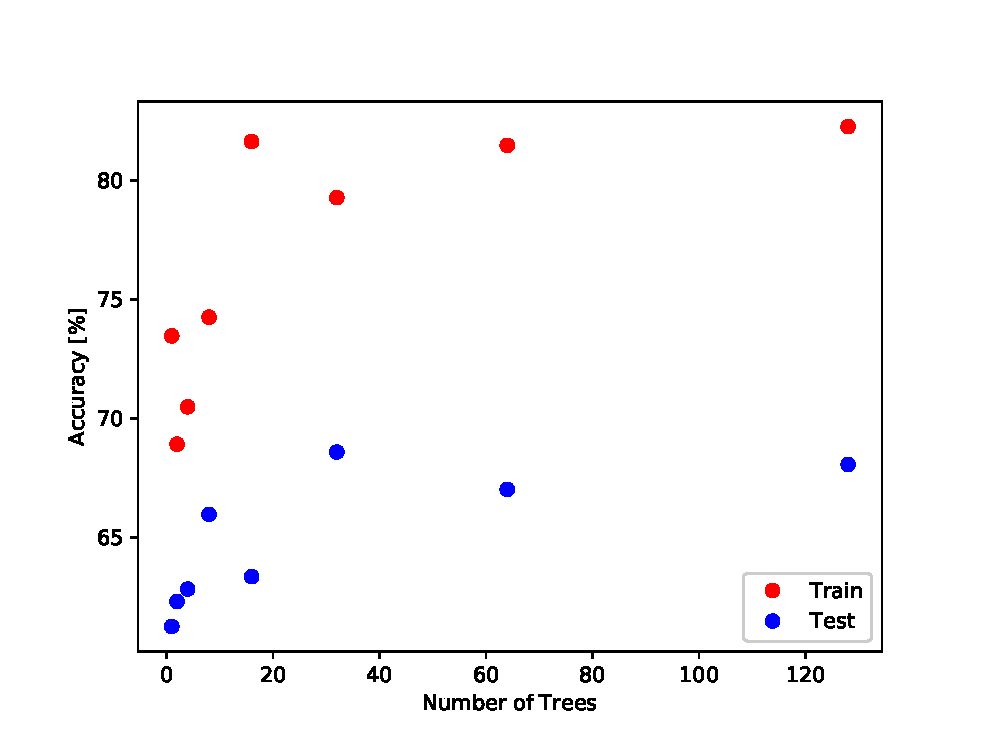
\includegraphics[scale=0.4]{n_trees}
%\framebox[4.0in]{$\;$}
%\fbox{\rule[-.5cm]{0cm}{4cm} \rule[-.5cm]{4cm}{0cm}}
\end{center}
\caption{Showing random forest inhibition to produce over fitting errors even with increased complexity by large number of trees.}
\label{fig:n_trees}
\end{figure}

The ability of random forests to resist over fitting is largely due to the number of trees and features, which is demonstrated in Figure ~\ref{fig:n_trees}. Randomization increases bias but makes it possible to reduce the variance of the corresponding ensemble model through averaging. \cite{formann-roe_2012}

\subsubsection{Tree Depth}

The depth of each decision tree used to make up the ensemble used in random forests has a large impact on the accuracy of the model. We investigate this by comparing the accuracy of our model implementation as a function of the maximum depth of each tree. That is, the tree can have a depth that is less than this value, depending on the features used to build the tree, however once it reaches this maximum depth, the leaf is forced to be a terminal and predict the target class. We keep other parameters such as number of trees, number of features, and minimum split size constant, with values 64, 5, 2 respectively.

\begin{figure}[ht]
\begin{center}
%\AddToShipoutPicture see eso-pic
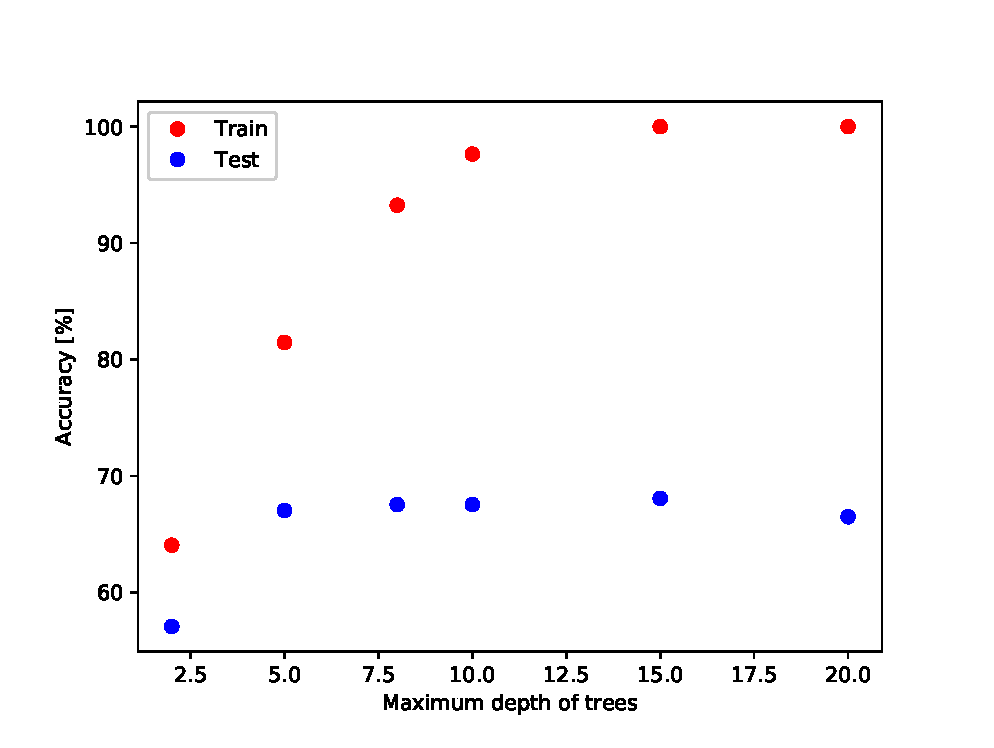
\includegraphics[scale=0.4]{max_depth}
%\framebox[4.0in]{$\;$}
%\fbox{\rule[-.5cm]{0cm}{4cm} \rule[-.5cm]{4cm}{0cm}}
\end{center}
\caption{Showing accuracy of random forest with 64 trees with varying maximum depth of each decision tree. It should be noted that there is a slight decrease in the test accuracy at 20 features which can possibly be related to over fitting on the training data which reaches 100\% after 15.}
\label{fig:max_depth}
\end{figure}

It has been shown that by increasing the maximum depth of each tree, a level of over fitting can be present, and similarly, having shallow trees can produce low-confidence predictions. \cite{Criminisi2011} It is thus important that an appropriate value of the maximum depth be used, as its optimal value is related to the problem complexity. We notice a small decrease in the accuracy at 20 features, as shown in Figure ~\ref{fig:max_depth} which suggests that random forests are still susceptible to over fitting, albeit less sensitive than many other machine learning algorithms without active regularization.

\subsubsection{Features Per Tree}

It is discussed in literature that an optimal value for the number of features to be used is $\frac{\text{ln}(M)}{\text{ln}(2)}$ of the total number of features, M. \cite{Brieman01} To investigate this we compare the classification accuracy while varying the number of features, with all other parameters such as number of trees, maximum depth, and minimum split size constant, with values 64, 5, 2 respectively.

\begin{figure}[ht]
\begin{center}
%\AddToShipoutPicture see eso-pic
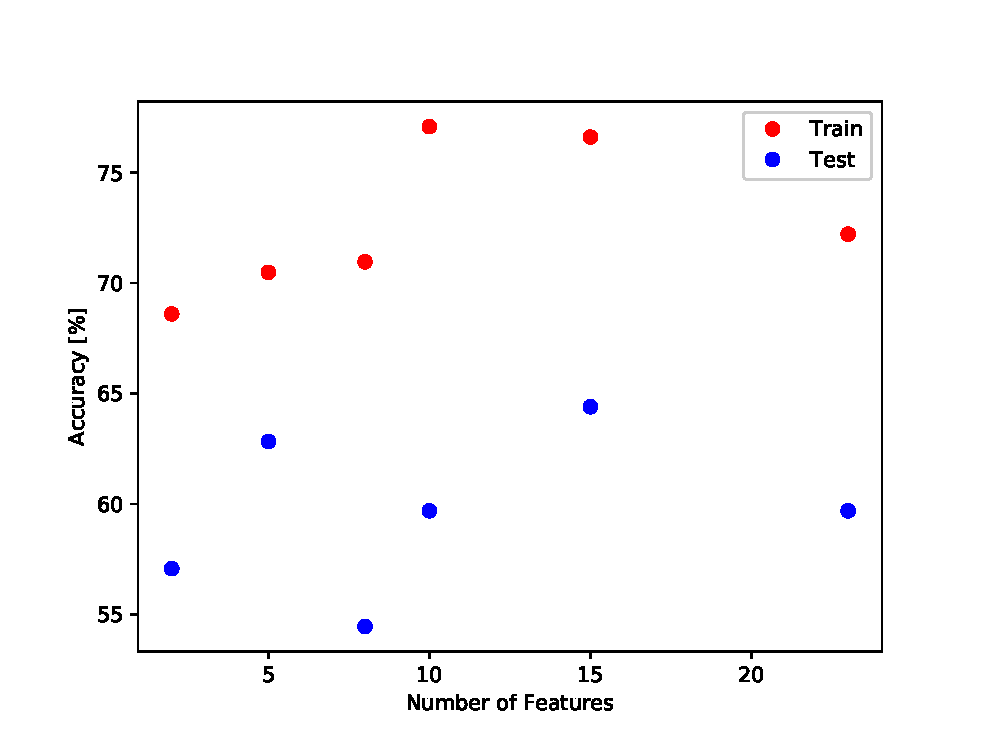
\includegraphics[scale=0.4]{n_features}
%\framebox[4.0in]{$\;$}
%\fbox{\rule[-.5cm]{0cm}{4cm} \rule[-.5cm]{4cm}{0cm}}
\end{center}
\caption{Showing the impact of the number of features used when constructing decision trees in random forest with 64 trees and max depth 5.}
\label{fig:n_features}
\end{figure}

Following our results, shown in figure ~\ref{fig:n_features}, we observe a maximum train accuracy for 5 features, which agrees with literature for an optimal number of features. We observe, however, that the number of features used has less of an impact on the total accuracy when comparing to the above observations for varying number of trees and maximum tree depth. The maximum depth for optimal test accuracy also does not agree with the training value, and the variance between each run makes drawing a conclusion on the over-all impact of this parameter difficult.

\subsubsection{Grid Search Parameter Optimization}

Following the observations after varying each parameter individually, a grid search method was employed to find the optimal values for number of trees, maximum depth, and number of features for our implementation of random forest. The range of values used for the grid search were as follows:

\begin{description}
\item [Trees] 2,8,16,32,64,128
\item [Depth] 2,5,8,10,15,20
\item [Features] 2,5,8,10,15,23
\end{description}

With optimal values shown in table ~\ref{opt-table}. Figure ~\ref{fig:gridSClass} shows the effect of the different parameters on the accuracy of the classifier for the test set. As can be observed, there are some local regions of high accuracy. In particular, when looking at the number of features for values $\frac{\text{ln}(M)}{\text{ln}(2)}$ which in this case correspond to a value of approximately 5. It is surprising that the optimal number of features is very low with a value of 2. This may be a result of creating a higher chance of uncorrelated trees which has been shown to improve accuracy. \cite{Bharathidason2014}

\begin{table}[h]
\caption{Optimal values found for project's random forest by grid search}
\begin{center}
\begin{tabular}{ccccc}
{\bf Target class} &{\bf Max depth} &{\bf Num features} &{\bf Num of trees}&{\bf Accuracy measure}
\\ \hline \\
GP\_greater\_than\_0         &15	&2	&64 &71.2\%\\
sum\_7yr\_GP         &5	&5	&2 		&11912\\
\label{opt-table}
\end{tabular}
\end{center}
\end{table}

\begin{figure}[ht]
%\AddToShipoutPicture see eso-pic
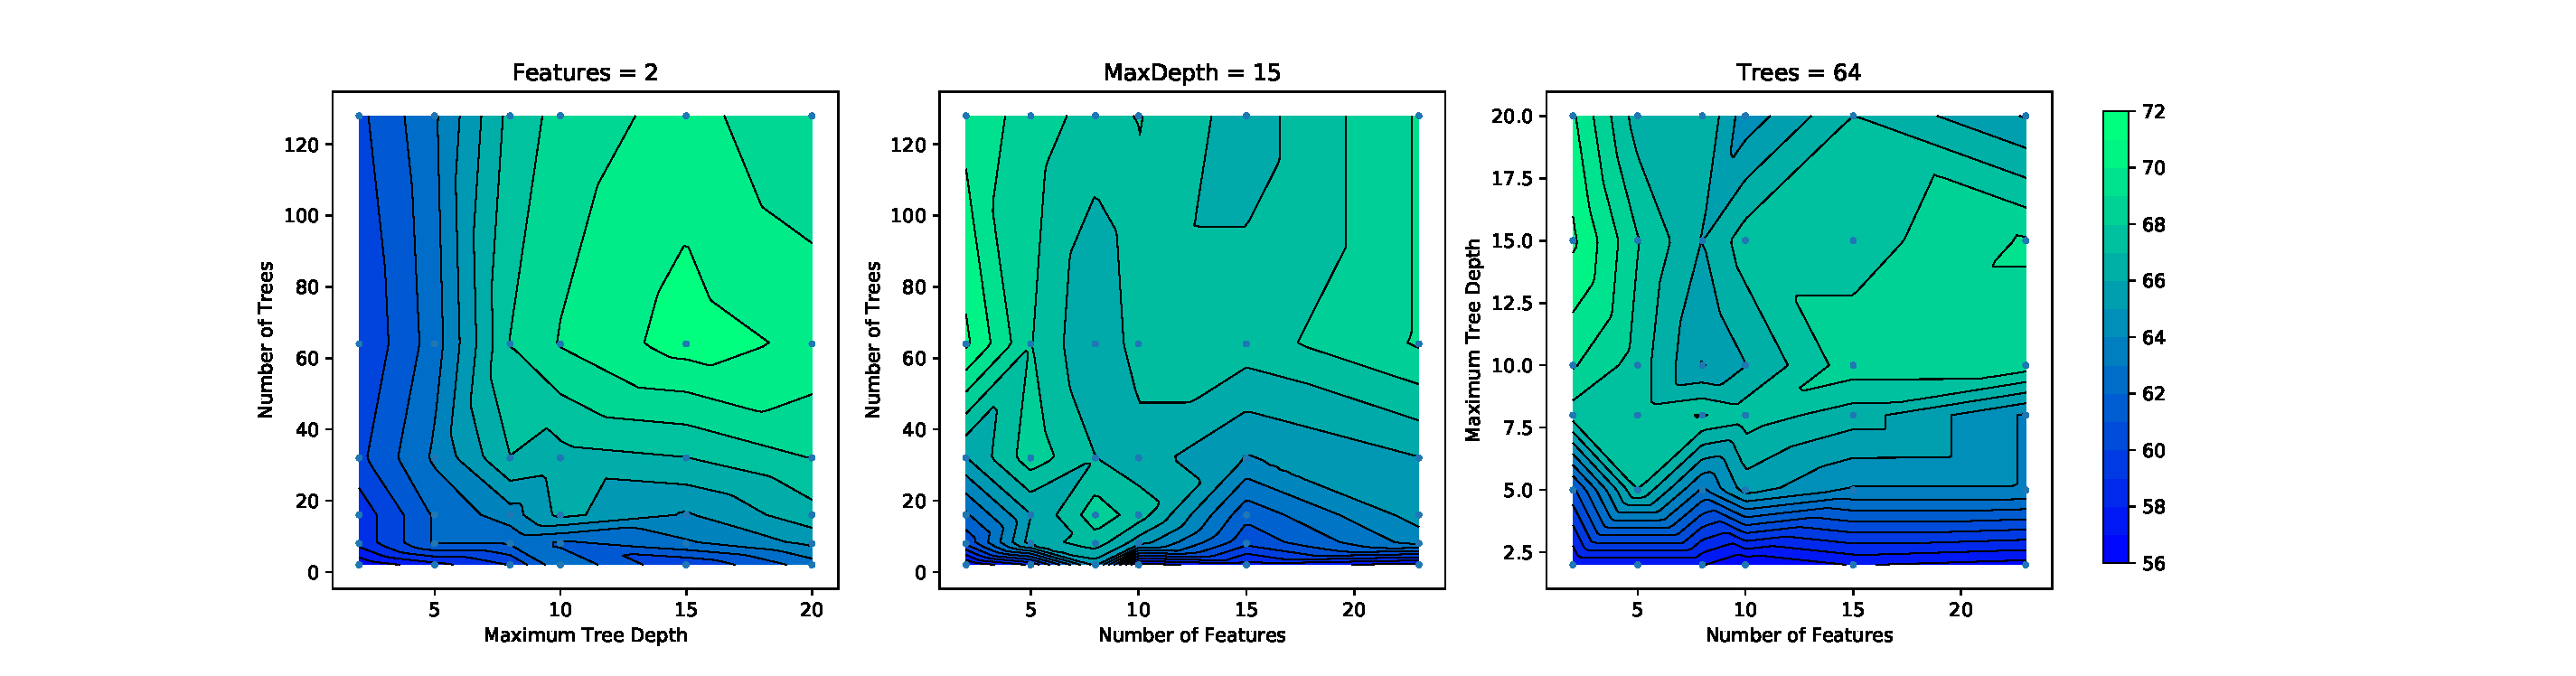
\includegraphics[width=1.1\textwidth]{gridSClass}
%\framebox[4.0in]{$\;$}
%\fbox{\rule[-.5cm]{0cm}{4cm} \rule[-.5cm]{4cm}{0cm}}
\caption{Showing results from grid search with effect on test set accuracy of project's random forest implementation}
\label{fig:gridSClass}
\end{figure}

\begin{table}[h]
\caption{Optimal values found for sci-kit learn random forest by grid search}
\begin{center}
\begin{tabular}{ccccc}
{\bf Target class} &{\bf Max depth} &{\bf Num features} &{\bf Num of trees}&{\bf Accuracy measure}
\\ \hline \\
GP\_greater\_than\_0         &8	&5 &128 &67.5\%\\
sum\_7yr\_GP         &8	&5 &64 &9270.5\\
\label{scikit-table}
\end{tabular}
\end{center}
\end{table}

Comparing the project's implementation of random forest to that of scikit-learn implementation, we further compare against the optimal values found by grid search, shown in table ~\ref{scikit-table}, and ~\ref{opt-table}. As can be seen, the values are quite different, although result in similar accuracy. A high number of trees is consistent between both showing the over-all effect of the random forest algorithm on improving performance for the classifier implementation. The difference between the values can be due to the different algorithms used and shows that finding optimal values for the specific algorithm is an important consideration when running any machine learning algorithm implementation. Using optimal values for learning, time for 4 processes of 20seconds is a significant improvement over a single process taking 1min 4sec for training GP\_greater\_than\_0, and comparing to table ~\ref{clas-table} the effect of increasing the number trees can be seen in the difference in time. After training however, prediction time is considerably lower, taking $\approx$1sec regardless. When training on sum\_7yr\_GP for a regression tree implementation, we note a considerable difference in both values and performance. The difference may be a result of the splitting criteria or bagging method, where by the average prediction is used for our implementation. From investigating the scikit-learn source code, it may be that there is also an additional degree of freedom where by each tree may have a different maximum depth which may also reduce the correlation between trees. The performance of an ensemble learner is dependent on the accuracy of each component learner and the diversity of the components, especially when using a small set of trees which may be limited due to computational cost. The randomization can cause occurrence of bad predicting trees as well as correlated trees which can lead to poor ensemble decisions, which can be observed when performing multiple training runs using the same parameters which can lead to different accuracy results. Attempts have been made to improve the performance of this model by building a forest of only uncorrelated high performing trees. \cite{Bharathidason2014}

\subsubsection{Splitting criteria}

When building a decision tree, the splitting criteria by which each level is formed to yield the greatest information gain can be calculated by two common methods; Entropy and Gini impurity. It has been discussed in literature that there exists a minimal difference between the effect of accuracy, however Gini
impurity function is computationally less expensive than Entropy since Entropy requires additionally calculating the logarithm of percentage of each class labels in the child nodes. The difference between the splitting criteria is investigated through the implementation of both entropy and Gini impurity in our implementation of random forest, with results shown in table ~\ref{ent-gini}. Both models were run on a single process.

\begin{table}[h]
\caption{Comparison of Entropy and Gini impurity for splitting criteria}
\begin{center}
\begin{tabular}{cccc}
{\bf Number of trees} &{\bf Gini impurity} &{\bf Entropy}
\\ \hline \\
4	&1min 23secs    &1min 47secs\\
16	&3min 58secs    &4min 26secs\\
32	&6min 19secs    &7min 23secs\\
\label{ent-gini}
\end{tabular}
\end{center}
\end{table}

As shown in table ~\ref{ent-gini}, using the Gini index as the score function is indeed noticeably faster than Entropy.


\subsection{Machine Learning Algorithm Comparisons}
TODO:  This section should be comparing our accuracy using best parameters against the best accuracy of other machine learning algorithms (e.g. linear regression, single decision trees, naive bayes, etc.)  
Needs to be more discussion here. It is simply a list with no explanation on why the difference. Why is SVM so low? Comparison of regression results?

For comparison, a decision tree classifier and a Support Vector Machine (SVM) were fitted and tested on the data. The test set accuracy of the decision tree was 64\% while the test accuracy of the SVM was 53\%.

\section{Conclusion}

Random forests have been shown to achieve high classification performance through ensemble with a set of decision trees that are constructed using randomly selected features. To investigate random forest we constructed the algorithm from scratch to provide the ability to better understand the impact of parameters and splitting methods. We compared our algorithm to two common machine learning libraries; Weka and Scikit-Learn. Using somewhat arbitrary values, we demonstrated that our algorithm is able to predict with similar accuracy and that the implementation is correct. Next we were able to explore the effect of parameters individually, by holding others constant. For simplicity we only considered the classifier type for this. We noted that there was an improvement with added number trees and also that typical overfitting was not observed as the complexity was increased, unlike many other machine learning algorithms. We did note however, that the maximum depth parameter can be used as regularization where we saw slight overfitting at a high number, which was consistent with discussion in literature. Following this, we then investigated varying all parameters to find optimal values. We noted that some surprising results emerged, where by the number of features for maximum accuracy for classification was only 2. This may have been a result on creating uncorrelated trees where there is low chance of having similar features used in this case. The implementation of regression trees however did not show a significant improvement in accuracy following gridsearch to obtain optimal values for parameters. This may be a result of the splitting criteria used for this implementation and warrants further investigation. Finally we compared the random forest algorithm to other machine learning algorithms. For a single decision tree the accuracy was indeed lower as well as for SVM (overfitting?)
From our experiments we observed several areas where improvement can be made in future work. The running time can be decreased by optimizing split function subroutines and the data structures to use Cython or C.
TODO: FINISH THIS PARAGRAPH

\subsubsection*{Contributions}
All authors contributed equally.\\
See GitLab repository here for specific commits:\\
\href{
    https://csil-git1.cs.surrey.sfu.ca/rkm3/mlclass-1777-randomforest
}{
    https://csil-git1.cs.surrey.sfu.ca/rkm3/mlclass-1777-randomforest
}


\small{
\bibliography{report}
\bibliographystyle{ieeetr}
}

\end{document}
